\documentclass[12pt]{article}

\usepackage[utf8]{inputenc}
\usepackage[T1]{fontenc}
\usepackage[spanish]{babel}
\usepackage{graphicx}
\usepackage{listings}
\usepackage{caption}
\usepackage{subcaption}
\usepackage[right=2cm,left=2cm,top=2cm,bottom=2cm]{geometry}
\usepackage{hyperref}
\usepackage{fancyhdr}
\usepackage{color}
\usepackage[export]{adjustbox}
\usepackage{graphicx}
\usepackage{float}
\usepackage{changepage}
\usepackage{multicol}
\usepackage{imakeidx}
\usepackage[spanish]{babel}
\usepackage[backend=biber]{biblatex}

\pagestyle{fancy}
\renewcommand{\footrulewidth}{0.4pt}
\setlength{\headheight}{15pt}


\fancyhead[L]{ CEIABD – MIA }
\fancyhead[R]{ Páez Anguita, Víctor }
\fancyfoot[L]{IES Gran Capitán}


\begin{document}

\begin{titlepage}
    \begin{center}
      \Large \bfseries{}
    \end{center}
    \vspace{0.1cm}
    \begin{center}
      \Large \bfseries{}
    \end{center}
    \vspace{0.1cm}
    \begin{center}
     \Large \bfseries{Sistema PLM}
    \end{center}
    \vspace{0.0001cm}
    \begin{center}
        Departamento de informática \\ I.E.S. Gran Capitán - Córdoba
    \end{center}
        \vspace{2 cm}
\begin{figure}[h!]
    \centering
    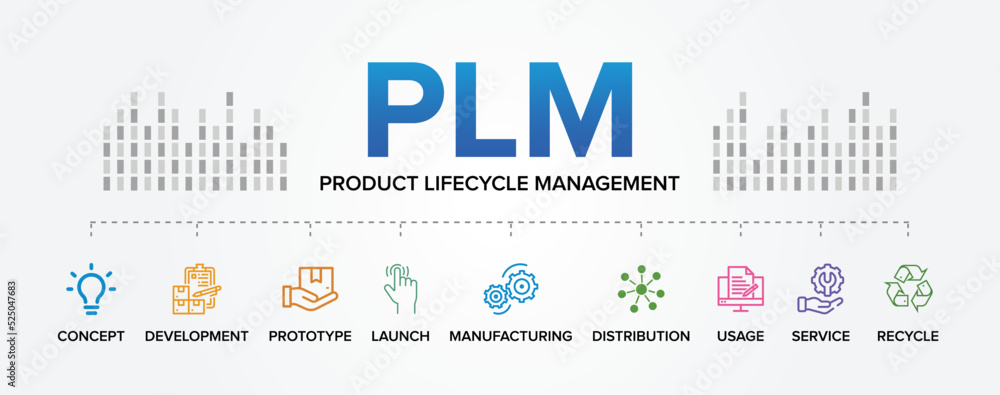
\includegraphics[width=.8\textwidth]{PLM.jpg}
    \label{fig:my_label}
\end{figure}
    \vspace{0.2 cm}
    \begin{center}
        Inteligencia artificial y Big data \\ Córdoba, 27 de Octubre 2024
    \end{center}
    \vspace{4 cm}
\null\hfill \textbf{Desarrollado por:}
\\
\\
\null\hfill Víctor Páez Anguita
\clearpage
\end{titlepage}

%%%%%%%%%%%%%%%%%%%%%%%%%%%Index%%%%%%%%%%%%%%%%%%%%%%%%%%%%%%%%
\tableofcontents
\clearpage
%%%%%%%%%%%%%%%%%%%%%%%%%%%Index%%%%%%%%%%%%%%%%%%%%%%%%%%%%%%%%

\section{Introducción}
En un nivel más básico, la gestión del ciclo de vida del producto (PLM) es el proceso estratégico de gestionar el viaje completo de un producto desde la idea inicial, 
el desarrollo, el servicio y la eliminación de desechos. Dicho de otra manera, PLM significa administrar todo lo relacionado con un producto desde la cuna hasta la tumba.

\section{Sistema PLM}

El software de PLM gestiona toda la información y procesos a lo largo del ciclo de vida de un producto en cadenas de suministro globales. Este incluye datos sobre artículos,
piezas, documentos, órdenes de cambio y flujos de trabajo de calidad. Con el crecimiento de las cadenas de suministro globalizadas y el cambio hacia modelos como producto 
como servicio (PaaS), las empresas necesitan soluciones de PLM en la nube para adaptarse rápidamente. El PLM moderno es fundamental en la transformación empresarial, 
permitiendo alinear la cadena de valor del producto con la planeación y ejecución, impulsando así la innovación y mejorando el diseño, fabricación, mantenimiento y servicios del producto.

\subsection{Características}
\begin{itemize}
    \item Gestión de documentos de diseño y procesos
    \item Gestión de configuración de BOM permitiendo variabilidad para sustentar el alcance completo de la configuración de un producto
    \item Visor incorporado que permite al usuario visualizar y manipular diseños de productos en 3D
    \item Estructura organizacional de compañía definida lo que permite control de acceso designado
    \item Flujos de trabajo digitales automatizados diseñados para capturar procesos de negocio en los que los documentos, información o tareas se pasan de un usuario a otro
    Amplias capacidades de reportes
    \item Integrado con herramientas de simulación
    \item Integrado con otros procesos de negocios tales como Gestión de Recursos Empresariales (Enterprise Resource Planning – ERP) y Sistemas de Ejecución de Manufactura (MES)
\end{itemize}

\subsection{Funciones}

\begin{enumerate}
    \item Concepto y diseño: la fase de ideación, donde los requisitos de un producto se definen en función de factores como el análisis de la competencia, 
    las brechas en el mercado o las necesidades del cliente.
    \item Desarrollar: Se creará el diseño detallado del producto, junto con cualquier diseño de herramientas necesario. Esta fase incluye la validación y el 
    análisis del producto planificado, así como el desarrollo de prototipos y el pilotaje en el campo. Esto genera un feedback vital sobre cómo se utiliza el producto y qué otros ajustes se necesitan.
    \item Concepto y diseño: la fase de ideación, donde los requisitos de un producto se definen en función de factores como el análisis de la competencia, las brechas en el mercado o las necesidades 
    del cliente.
    \item Producción y lanzamiento: El feedback del piloto se utiliza para ajustar el diseño y otros componentes para producir una versión lista para el mercado. La producción del nuevo producto se escala, 
    seguido del lanzamiento y la distribución al mercado.
    \item Servicio y soporte: Tras el lanzamiento del nuevo producto, el período de tiempo en el que se ofrece el servicio y el soporte.
    \item Retiro: Al final del ciclo de vida del producto, su retirada del mercado debe gestionarse, junto con cualquier recuperación o absorción en nuevas ideas conceptuales.
\end{enumerate}

\begin{figure}[h!]
    \centering
    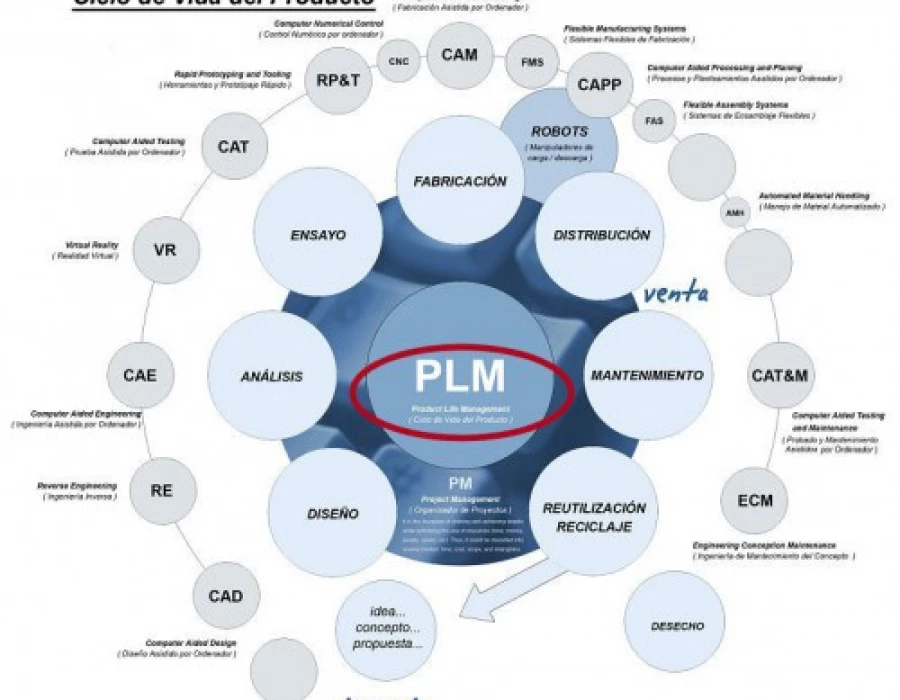
\includegraphics[width=.8\textwidth]{Funciones.jpg}
    \label{fig:my_label}
\end{figure}

\subsection{Arquitectura}


La arquitectura de un sistema PLM (Product Lifecycle Management) suele basarse en una estructura de múltiples capas que permite gestionar y 
conectar de manera eficiente toda la información y procesos relacionados con el ciclo de vida del producto. Esta arquitectura generalmente 
incluye las siguientes capas y componentes:

\begin{itemize}
    \item Capa de Presentación (Interfaz de Usuario)
    \item Capa de Aplicación (Lógica de Negocio)
    \item Capa de Servicios de Integración
    \item Capa de Datos (Base de Datos)
    \item Capa de Seguridad
    \item Capa de Infraestructura (Nube o Servidor)
\end{itemize}

Por otra parte podemos diferenciar dos tipos de arquitecturas PLM:
\begin{itemize}
    \item PLM en la nube: Ofrece flexibilidad y escalabilidad, permitiendo a las empresas ajustarse a las necesidades del mercado
    y conectarse con equipos globales en tiempo real.
    \item PLM en servidor local: Brinda mayor control y personalización, pero puede ser más costoso y menos flexible en cuanto a 
    accesibilidad y actualizaciones.
\end{itemize}

\section{Diferencia entre un sistema ERP y PLM}

PLM y ERP son dos tipos de sistemas de gestión usados en las empresas, cada uno con un enfoque y objetivo específico. Mientras que PLM se centra en gestionar los datos y procesos relacionados con los 
productos durante todo su ciclo de vida, desde su diseño inicial hasta su retiro, los sistemas ERP están orientados a administrar diversas operaciones comerciales, como las finanzas, recursos humanos 
y la cadena de suministro. Aunque ambos sistemas gestionan datos importantes para la empresa, sus funcionalidades y enfoques son distintos.
Para entender mejor la diferencia, es útil observar el alcance de cada sistema. PLM está más orientado hacia el diseño, la fabricación y el mantenimiento de productos, priorizando la innovación y 
la creatividad. En cambio, ERP se ocupa de los procesos comerciales principales, como las finanzas, ventas y la fabricación.
En cuanto al tipo de datos que manejan, los sistemas PLM se ocupan de los datos de productos, de ingeniería y de fabricación. Los sistemas ERP, en cambio, gestionan datos financieros, información de 
clientes e inventarios. Estas diferencias reflejan las distintas prioridades y objetivos de cada sistema.
 \\
 \\
 En la siguiente imagen podemos observar con más claridad la diferencia entre ambos sistemas:
\begin{figure}[h!]
    \centering
    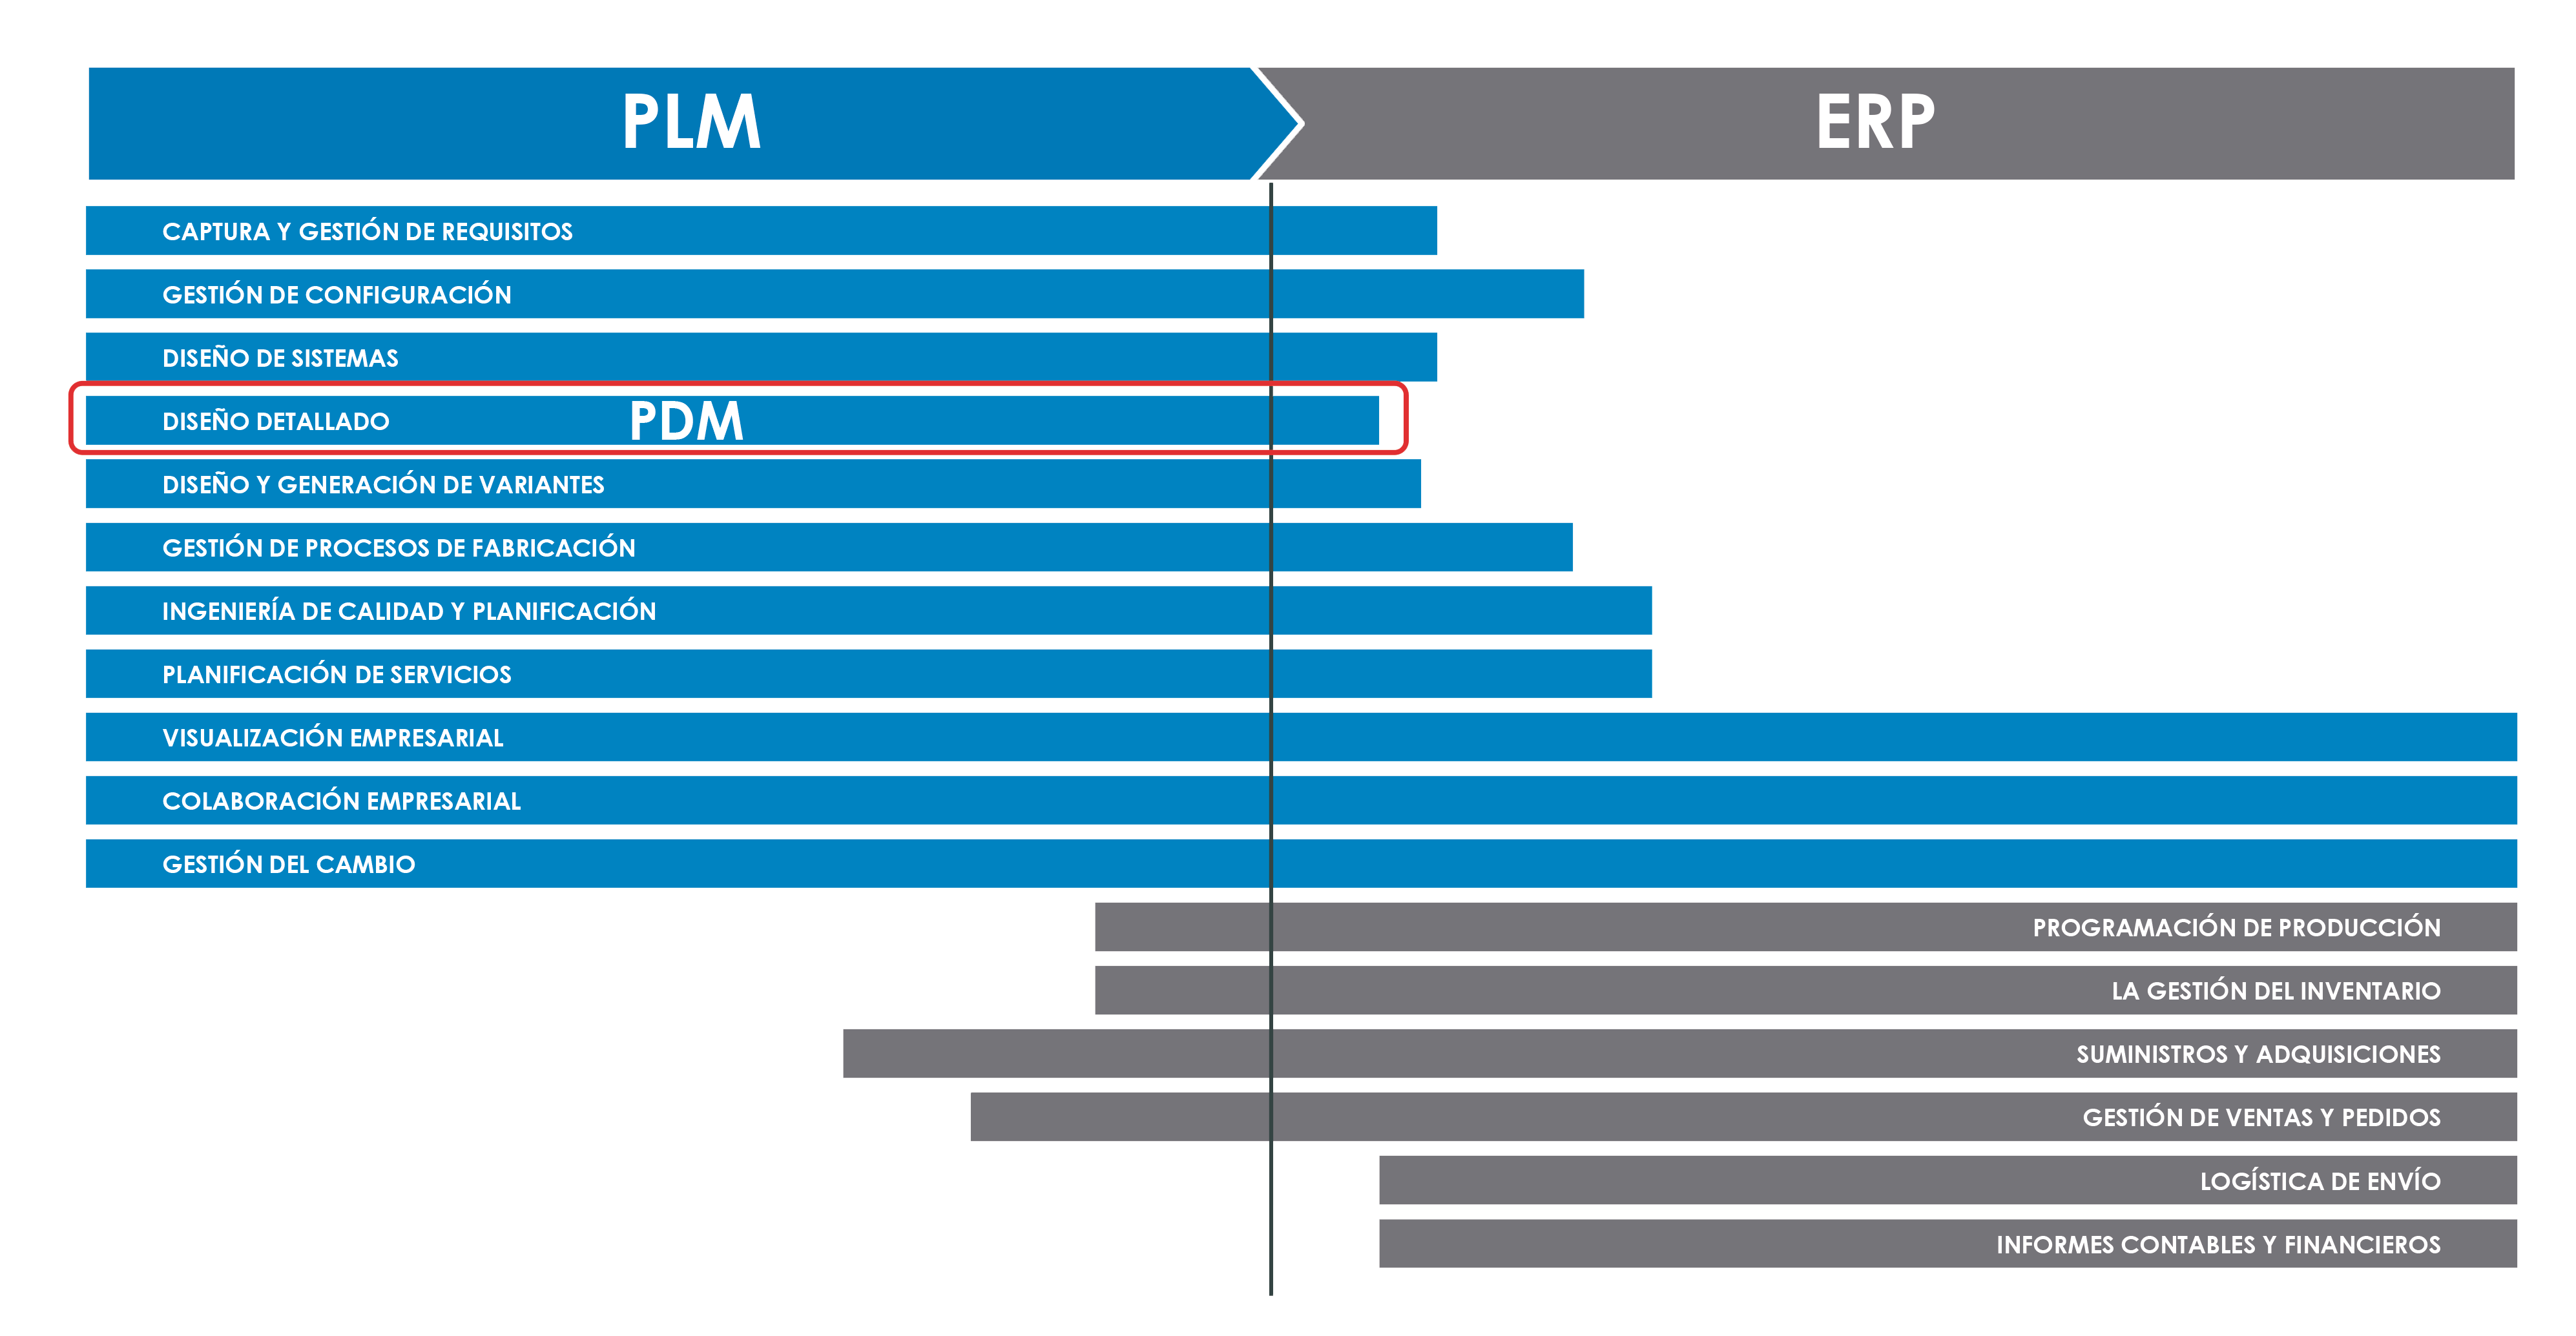
\includegraphics[width=.7\textwidth]{esquema-plm-pdm-erp.png}
    \label{fig:my_label}
\end{figure}

\clearpage

\section{Empresas que ofrecen sistemas PLM}

\subsection{Oracle}

Fusion Cloud Product Lifecycle Management ofrece una herramienta para seguir los productos desde la innovación hasta la producción e incluso la venta. El objetivo es crear un bucle cerrado 
virtuoso para la colaboración con los miembros del equipo basado en los datos recogidos de las pruebas, las líneas de producción y los informes de ventas. La sección de MDM recopilará datos 
del marketing omnicanal, los canales de venta, los canales ERP y los proveedores externos de la cadena de suministro. El objetivo es un proceso de toma de decisiones bien orquestado con funciones, 
responsabilidades y gobernanza bien definidas.

\subsection{SAP}

La solución de SAP para PLM está bien integrada con el sistema de gestión de SAP, que organiza los almacenes y los centros de distribución. Las herramientas de gestión de carteras y 
productos se centran en la creación de entornos de colaboración fluidos para el diseño de nuevos productos, la estimación precisa de los costes de producción y la previsión de los problemas de 
cumplimiento. La integración financiera ayuda a garantizar que el producto final no sea sólo un deleite visual, sino un éxito económico que llegue a tiempo. Los gastos de capital, el modelado de 
la capacidad y los costes de I+D entran en la ecuación para el seguimiento del proyecto.

\section{Ejemplos reales de uso de sistemas PLM en empresas y su repercusión}

\subsection{Boeing}
\begin{itemize}
    \item Uso de PLM: Boeing utiliza Dassault Systèmes ENOVIA, un sistema PLM, para el diseño y desarrollo de sus aviones, incluyendo la gestión de componentes, 
    materiales y procesos de producción.
    \item Repercusión: ENOVIA ha ayudado a Boeing a gestionar con precisión los complejos datos de ingeniería de cada avión. Con este sistema, 
    Boeing ha mejorado la colaboración entre diferentes departamentos y proveedores en todo el mundo, lo que permite optimizar el flujo de trabajo y 
    reducir tiempos de producción. Además, al centralizar la información en una plataforma digital, la empresa ha minimizado errores costosos en el 
    ensamblaje y fabricación de componentes.
\end{itemize}

\subsection{Coca-Cola}
\begin{itemize}
    \item Uso de PLM: Coca-Cola implementó el sistema PLM Infor Optiva para mejorar la gestión de formulaciones y recetas.
    \item Repercusión: Gracias a este sistema, Coca-Cola ha optimizado la gestión de fórmulas y el desarrollo de nuevos productos. 
    La implementación de PLM le ha permitido reducir los costos de desarrollo y asegurar que sus productos cumplan con las normativas 
    locales en cada país. Además, ha mejorado la trazabilidad de ingredientes, ayudando a la empresa a gestionar de forma más eficiente 
    los recursos y a responder rápidamente a cambios en las regulaciones o en las demandas de los consumidores.
\end{itemize}

\section{Empresas que han utlizado sistema PDM con éxito}

\subsection{Ford Motor Company}
Ford implementó un sistema de PDM para mejorar la gestión de datos de diseño y la colaboración en el desarrollo de nuevos vehículos.
\\
La solución de PDM permitió a Ford centralizar y gestionar de manera eficaz la gran cantidad de datos generados durante el diseño y 
desarrollo de sus vehículos. Gracias al PDM, los ingenieros y diseñadores de Ford pueden acceder a versiones actualizadas de los archivos 
en tiempo real, lo cual minimiza errores de duplicación y permite una revisión y aprobación más rápida de los diseños. Como resultado, 
Ford ha reducido significativamente el tiempo de desarrollo de nuevos modelos y ha aumentado la calidad de sus productos al mejorar la 
comunicación entre equipos.

\subsection{Caterpillar Inc.}
Caterpillar implementó un sistema de PDM para gestionar los datos de diseño de sus productos de maquinaria pesada.
\\
El PDM permitió a Caterpillar unificar y gestionar la información de los productos de manera centralizada, lo cual fue clave para la 
colaboración entre los equipos de diseño, ingeniería y producción en múltiples ubicaciones. El sistema de PDM ayudó a mejorar la trazabilidad 
de los datos y la eficiencia en el control de versiones, evitando costosos errores en la fabricación. Esto redujo el tiempo y los costos de 
producción, ayudando a Caterpillar a lanzar nuevos productos al mercado de manera más ágil y competitiva.

\clearpage

\section{Bibliografia}
\begin{itemize}
    \item \href{https://www.oracle.com/es/scm/product-lifecycle-management/what-is-plm/}{Oracle}.
    \item \href{efaidnbmnnnibpcajpcglclefindmkaj/https://ria.utn.edu.ar/bitstream/handle/20.500.12272/4420/SISTEMAS%20PLM.pdf?sequence=1&isAllowed=y}{RIA-UTN}.
    \item \href{https://www.indx.com/es/solution/product-lifecycle-management-plm-for-discrete-industry}{ENG}
    \item \href{https://www.sap.com/spain/products/scm/plm-r-d-engineering/what-is-product-lifecycle-management.html}{SAP}
    \item \href{https://deplm.com.ar/siemens-plm/diferencias-entre-plm-y-erp/}{deplm}
    \item \href{https://www.cio.com/article/2071332/los-15-mejores-proveedores-de-plm.html}{CIO}
    \item \href{https://es.ford.com/}{Ford}
    \item \href{https://www.coca-cola.com/es/es}{Coca-Cola}
    \item \href{https://www.boeing.es/}{Boeing}
    \item \href{https://www.caterpillar.com/es.html}{Caterpillar Inc.}

\end{itemize}

\end{document}
